\documentclass[12pt]{article}
\usepackage[margin=1.5cm]{geometry}
\usepackage{parskip}
\usepackage{amsmath}
\usepackage{amssymb}
\usepackage{amsfonts}
\usepackage{enumitem}
\usepackage{graphicx}
\usepackage{stmaryrd}
\graphicspath{ {./images/} }


\begin{document}
The Needleman-Wunsch algorithm is a sequence alignment algorithm.

The sequence alignment problem is the problem of finding the best alignment between two sequences such that regions of similarity are conserved. For example, this can help to find similarities between DNA sequences of two different species.

In particular, the Needleman-Wunsch algorithm solves the global alignment problem, which is where we align two entire strings against each other.

The algorithm is a dynamic programming algorithm, so if we are trying to align two sequences $x$ and $y$, if we have alignments of prefixes of $x$ and $y$, we can align these prefixes plus 1 character, for example.

The algorithm takes as input two strings $x, y$, a gap penalty $\delta$, and a scoring matrix $s$ (which gives the match/mismatch score between two characters), and returns as output an alignment score and alignment.

Then, we compute the following function/matrix with dynamic programming:

\[
  F(i,j) = \max\begin{cases}F(i-1, j) - \delta\\F(i, j-1) - \delta\\F(i-1, j-1)+ s(x_i, y_j)\end{cases}
.\] 

With initialisation of $F(i,0) = -i \cdot \delta$ and $F(0, j) = -j \cdot \delta$ for all $i$ and $j$.

We also store an additional $Ptr$ matrix that tells us in what direction to go to trace back an alignment.

Then, we get the alignment score in $F(|x|, |y|)$, and backtrack using the $Ptr$ matrix to obtain an alignment.

Consider the following example:

Suppose we are aligning DNA sequences $ACCAGT$ and $CCAGGT$, with $\delta = 1$ and $s(x_i, y_j) = 1$ if $x_i = y_j$, and $-2$ otherwise.

We build the following matrix:

\begin{tabular}{c|c|c|c|c|c|c|c}
  &$\omega$&A&C&C&A&G&T\\
  \hline
  $\omega$&0&-1&-2&-3&-4&-5&-6\\
  \hline
  C&-1&-2&0&-1&-2&-3&-4\\
  \hline
  C&-2&-3&-1&1&0&-1&-2\\
  \hline
  A&-3&-1&-2&0&2&1&0\\
  \hline
  G&-4&-2&-3&-1&1&3&2\\
  \hline
  G&-5&-3&-4&-2&0&2&1\\
  \hline
  T&-6&-4&-5&-3&-1&1&3
\end{tabular}

By backtracking from the bottom-right corner, we get the alignment:

\begin{verbatim}
ACCA-GT
-CCAGGT
\end{verbatim}

Note that this is a unique alignment, but sometimes there will be multiple alignments with the same alignment score.

A naive implementation of this algorithm has $O(nm)$ time complexity and $O(nm)$ space complexity to fill the matrix (where $n = |x|$ and $m = |y|$).

However, an optimisation exists to reduce the space complexity to $O(n)$ whilst keeping the time complexity at $O(nm)$. 

To see this optimisation, first note that we can compute the alignment score for two strings with only $O(n)$ space, since we only ever need one column worth of space at any given time, one that we are filling in, and another that we compute values from, so we can recycle this memory.

Then, notice that we can compute an alignment of two strings by first finding the unique node in the middle column that the alignment passes through, and recursively computing the alignment in the two subrectangles we create:

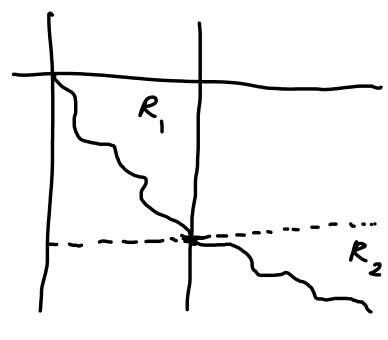
\includegraphics[scale=0.5]{middlenode}

To find this middle node, we can compute the alignment scores in the middle column in $O(n)$ space and $O(nm)$ time as before, and add this to the alignment scores in the middle column yielded by using the reverse edit graph, from the bottom right to the middle column, again in $O(n)$ space and $O(nm)$ time as before. The middle node will be the one which has the highest summed score.

This takes time proportional to the area, $nm$, but the recursive computations only have a quarter of the area each, so the total time complexity becomes $O(nm) \cdot \sum_{i=0}^\infty 2^{-i} = O(nm)$.

An optimisation also exists to improve the time complexity to $O(\frac{n^2}{\log n})$ with space complexity $O(n^2)$ (assuming that $n = \max(n,m)$ here for simplicity).

This is the Four Russians speedup. It works by dividing our matrix into a grid of blocks of size $t \times t$. We then create a lookup table that has pre-calculated alignments for each block. For each possible pairs of $t$-length sequences, we can compute their alignment and store it in a lookup table. Then, we compute an alignment through these blocks.

This lookup table will be of size $4^t \times 4^t$, so if $t = \frac{\log n}{4}$ it has size $n$.

Since we require $\frac{n}{t} \cdot \frac{n}{t}$ accesses in total, and each access takes $O(\log n)$ time, we get the total running time as $O(\frac{n^2}{\log n})$ time.

The algorithm makes the potentially unreasonable assumption that gaps should be penalised linearly, when in reality sequences of gaps likely occur in a single biological event, not a combination of them. So, we would like to use a concave gap penalty function, but this increases the time complexity to $O(n^3)$, so we make the tradeoff of using an affine gap penalty, which has a high gap opening penalty, but a small gap extension penalty.






\end{document}
